

\tikzset{every picture/.style={line width=0.75pt}} %set default line width to 0.75pt        

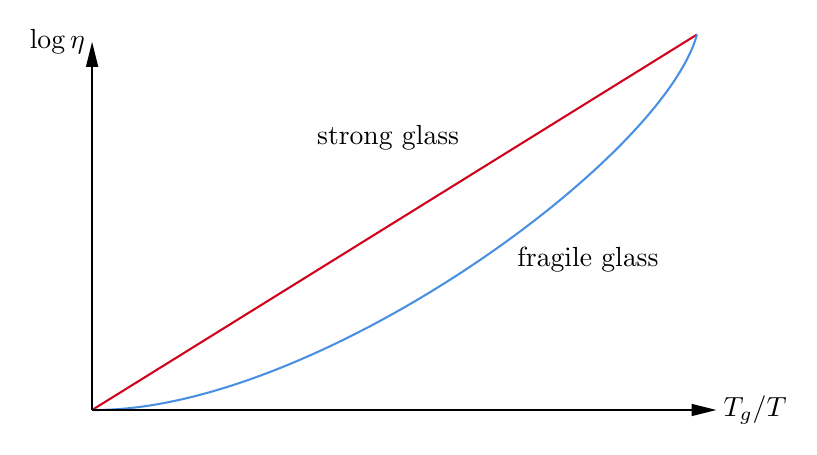
\begin{tikzpicture}[x=0.75pt,y=0.75pt,yscale=-1,xscale=1]
%uncomment if require: \path (0,300); %set diagram left start at 0, and has height of 300

%Straight Lines [id:da1597530183407554] 
\draw [color={rgb, 255:red, 208; green, 2; blue, 27 }  ,draw opacity=1 ]   (182,226.33) -- (473.43,45.44) ;
%Curve Lines [id:da7858735050814729] 
\draw [color={rgb, 255:red, 74; green, 144; blue, 226 }  ,draw opacity=1 ]   (182,226.33) .. controls (288.43,227.44) and (456.43,106.44) .. (473.43,45.44) ;
%Straight Lines [id:da13335799595525732] 
\draw    (182,226.33) -- (480.79,226.33) ;
\draw [shift={(482.79,226.33)}, rotate = 180] [fill={rgb, 255:red, 0; green, 0; blue, 0 }  ][line width=0.08]  [draw opacity=0] (12,-3) -- (0,0) -- (12,3) -- cycle    ;
%Straight Lines [id:da08630284642228214] 
\draw    (182,226.33) -- (182,51.06) ;
\draw [shift={(182,49.06)}, rotate = 450] [fill={rgb, 255:red, 0; green, 0; blue, 0 }  ][line width=0.08]  [draw opacity=0] (12,-3) -- (0,0) -- (12,3) -- cycle    ;

% Text Node
\draw (180,49.06) node [anchor=east] [inner sep=0.75pt]    {$\log \eta $};
% Text Node
\draw (484.79,226.33) node [anchor=west] [inner sep=0.75pt]    {$T_\text{g} / T$};
% Text Node
\draw (288.92,87.5) node [anchor=north west][inner sep=0.75pt]   [align=left] {strong glass};
% Text Node
\draw (385.42,146.5) node [anchor=north west][inner sep=0.75pt]   [align=left] {fragile glass};


\end{tikzpicture}
